
\section{Introduction}

Following are two examples of using randomLCA for latent class analysis. Some aspects will certainly change but most code should still work. Two things that will change are the use of accessor functions and better labelling of results.

\section{Latent Class}

\subsection{Model}

The basis of latent class analysis is that each subject belongs to one of a finite number of classes, with each class described by a set of parameters that define the distribution of outcomes or manifest variables for a subject, a form of finite mixture model. For binary outcomes, the model for each class is
\begin{eqnarray*}
P\left(y_{i1},y_{i2},...,y_{ik}\right|c)&=&\prod_{j=1}^k \pi_{cj}^{y_{ij}} \left(1-\pi_{cj}\right)^{1-y_{ij}}
\end{eqnarray*}
where
\begin{eqnarray*}
y_{ij}&=&\mbox{$j$th binary outcome for subject $i$}\\
\pi_{cj}&=&\mbox{probability of $j$th outcome equal to 1 for subject in class $c$}\\
k&=&\mbox{number of outcomes.}
\end{eqnarray*}

An additional parameter that is required to be estimated is $\eta_c$, the probability of a subjects in class $c$.

A requirement for the estimates of the probabilities $\pi_{cj}$ is that they be restricted to the interval zero to one, and $\eta_c$ sum to one. This can be obtained using the following relations $\pi_{cj}=\frac{e^{a_{cj}}}{1+e^{a_{cj}}}$ and $\eta_c=\frac{e^{\theta_c}}{\sum_{\ell=1}^C e^{\theta_\ell}}$. Hence we estimate the $\pi_{cj}$ and $\theta_c$.


\subsection{Example 1}


This example demonstrates the fitting of data from \citet{rindskopf:1986}, where latent class analysis is used to determine diagnostic classifications based on medical tests. Although this example is for medical data, the model is simply standard latent class so the methods can be applied to data from other areas.

A series of latent class models for 1 and 2 classes (any models with additional classes are not identifiable) can be fitted using the commands
\begin{Schunk}
\begin{Sinput}
> data(myocardial)
> myocardial.lca1 <- randomLCA(myocardial[,1:4],
+ 	freq=myocardial$freq,nclass=1)
> myocardial.lca2 <- randomLCA(myocardial[,1:4],
+ 	freq=myocardial$freq,nclass=2)
\end{Sinput}
\end{Schunk}

The BIC values may be extracted from the fitted objects and are shown in Table~\ref{tab:bic1}. 

\begin{Schunk}
\begin{Sinput}
> bic.data <- data.frame(classes=1:2,bic=c(BIC(myocardial.lca1),BIC(myocardial.lca2)))
\end{Sinput}
\end{Schunk}



% latex table generated in R 3.1.2 by xtable 1.7-3 package
% Mon Nov 17 10:15:10 2014
\begin{table}[ht]
\centering
\begin{tabular}{rr}
  \hline
classes & bic \\ 
  \hline
1 & 524.7 \\ 
  2 & 402.3 \\ 
   \hline
\end{tabular}
\caption{BIC by class.} 
\label{tab:bic1}
\end{table}


Using BIC as a selection method, this selects the 2 class model, indicating a nice beakdown into diseased and nondiseased, which it is assumed represent those with and without myocardial infarction. The true nature of classes is always debateable.

Summary may be used to display the fitted results

\begin{Schunk}
\begin{Sinput}
> summary(myocardial.lca2)
\end{Sinput}
\begin{Soutput}
  Classes      AIC      BIC    logLik penlogLik
        2 379.3958 402.2855 -180.6979 -180.7002
Class probabilities 
Class  1 Class  2 
  0.4578   0.5422 
Outcome probabilities 
         Q.wave History    LDH    CPK
Class  1 0.7668  0.7914 0.8279 1.0000
Class  2 0.0000  0.1951 0.0269 0.1955
\end{Soutput}
\end{Schunk}

Individual results may be obtained from summary, for example the outcome probabilities shown in Table~\ref{tab:outcomep1}.
\begin{Schunk}
\begin{Sinput}
> outcomep.data <- summary(myocardial.lca2)$outcomep
\end{Sinput}
\end{Schunk}



% latex table generated in R 3.1.2 by xtable 1.7-3 package
% Mon Nov 17 10:15:10 2014
\begin{table}[ht]
\centering
\begin{tabular}{rrrrr}
  \hline
 & Q.wave & History & LDH & CPK \\ 
  \hline
Class  1 & 0.767 & 0.791 & 0.828 & 1.000 \\ 
  Class  2 & 0.000 & 0.195 & 0.027 & 0.196 \\ 
   \hline
\end{tabular}
\caption{Outcome Probabilities.} 
\label{tab:outcomep1}
\end{table}


This gives some interesting information. In Class 2, those without myocardial infarction, will have abscence of Q.wave but in those with myocardial infarction it will only be present in 76.7\%. The class probabilities can be obtained as \texttt{myocardial.lca2\$classp} of 0.46 and 0.54 for Class 1 and 2 respectively.


One aspect of latent class is that no subject is uniquely allocated to a given class, although in some cases a subject may have an extremely high probability.

The posterior class probs can be obtained as

\begin{Schunk}
\begin{Sinput}
> classprobs <- post.classProbs(myocardial.lca2)
\end{Sinput}
\end{Schunk}

with results shown in Table~\ref{tab:classprob1}. This shows subjects with 3 or 4 positive tests to be strongly classified as having myocardial infarction, and even some with 2, depending on which to to be well classified. Having only one positive test makes it unlikely that it is myocardial infarction.



% latex table generated in R 3.1.2 by xtable 1.7-3 package
% Mon Nov 17 10:15:10 2014
\begin{table}[ht]
\centering
\begin{tabular}{rrrrrrr}
  \hline
Q.wave & History & LDH & CPK & Freq & Class 1 & Class 2 \\ 
  \hline
1 & 1 & 1 & 1 & 24 & 1.000 & 0.000 \\ 
  0 & 1 & 1 & 1 & 5 & 0.992 & 0.008 \\ 
  1 & 0 & 1 & 1 & 4 & 1.000 & 0.000 \\ 
  0 & 0 & 1 & 1 & 3 & 0.889 & 0.111 \\ 
  1 & 1 & 0 & 1 & 3 & 1.000 & 0.000 \\ 
  0 & 1 & 0 & 1 & 5 & 0.419 & 0.581 \\ 
  1 & 0 & 0 & 1 & 2 & 1.000 & 0.000 \\ 
  0 & 0 & 0 & 1 & 7 & 0.044 & 0.956 \\ 
  0 & 0 & 1 & 0 & 1 & 0.000 & 1.000 \\ 
  0 & 1 & 0 & 0 & 7 & 0.000 & 1.000 \\ 
  0 & 0 & 0 & 0 & 33 & 0.000 & 1.000 \\ 
   \hline
\end{tabular}
\caption{Class Probabilities.} 
\label{tab:classprob1}
\end{table}

Outcome probabilities are shown in Figure~\ref{fig:outcome2a}.

\begin{figure}
  \centering
\begin{Schunk}
\begin{Sinput}
> trellis.par.set(col.whitebg())
> print(plot(myocardial.lca2,type="l",xlab="Test",
+   ylab="Outcome Probability",scales=list(x=list(at=1:4,
+   labels=names(myocardial)[1:4]))))
\end{Sinput}
\end{Schunk}
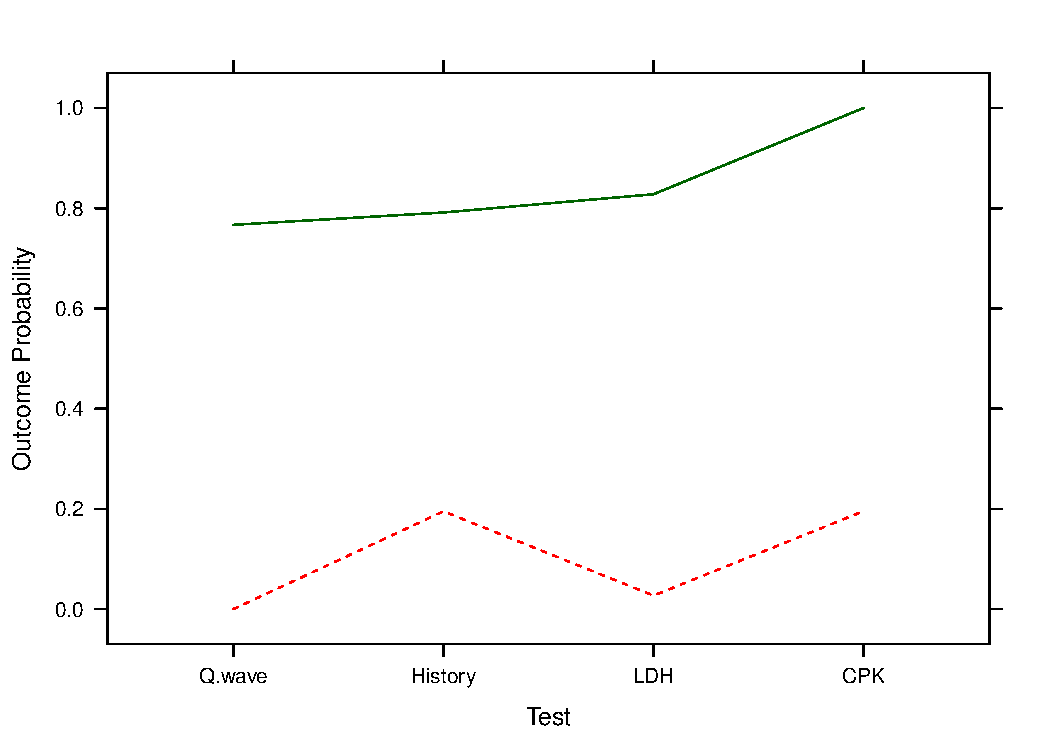
\includegraphics{randomLCA-example-010}
  \caption{Outcome probabilities for 2 Class Latent Class model.}
  \label{fig:outcome2a}
\end{figure}


\subsection{Example 2}

This example shows the fitting of the dentistry data from \citet{qu:1996}. The data consists of the results of five dentists evaluating x-rays for presence or absence of caries. As there is no gold standard, the latent class method is to assume two classes, diseased and non-diseased which are identified from the data.

A series of latent class models for 1 to 4 classes can be fitted using the commands
\begin{Schunk}
\begin{Sinput}
> data(dentistry)
> dentistry.lca1 <- randomLCA(dentistry[,1:5],
+ 	freq=dentistry$freq,nclass=1)
> dentistry.lca2 <- randomLCA(dentistry[,1:5],
+ 	freq=dentistry$freq,nclass=2)
> dentistry.lca3 <- randomLCA(dentistry[,1:5],
+ 	freq=dentistry$freq,nclass=3,quadpoints=31)
> dentistry.lca4 <- randomLCA(dentistry[,1:5],
+ 	freq=dentistry$freq,nclass=4,quadpoints=41)
\end{Sinput}
\end{Schunk}

The BIC values may be extracted from the fitted objects and are shown in Table~\ref{tab:bic}. This indicates the presence of 3 classes. A possible interpretation is that there is a class of subjects with moderate disease, or the alternative of heterogeneous disease which will be covered in the next section. Outcome probabilities are shown in Figure~\ref{fig:outcome3} and for the 2 class model in Figure~\ref{fig:outcome2b}.

\begin{Schunk}
\begin{Sinput}
> bic.data <- data.frame(classes=1:4,bic=c(BIC(dentistry.lca1),
+ 	BIC(dentistry.lca2),BIC(dentistry.lca3),BIC(dentistry.lca4)))
\end{Sinput}
\end{Schunk}




% latex table generated in R 3.1.2 by xtable 1.7-3 package
% Mon Nov 17 10:15:19 2014
\begin{table}[ht]
\centering
\begin{tabular}{rr}
  \hline
classes & bic \\ 
  \hline
1 & 17531.1 \\ 
  2 & 15021.6 \\ 
  3 & 14962.9 \\ 
  4 & 15000.0 \\ 
   \hline
\end{tabular}
\caption{BIC by class.} 
\label{tab:bic}
\end{table}


\begin{figure}
  \centering
\begin{Schunk}
\begin{Sinput}
> trellis.par.set(col.whitebg())
> print(plot(dentistry.lca3,type="l",xlab="Dentist",
+     ylab="Outcome Probability"))
\end{Sinput}
\end{Schunk}
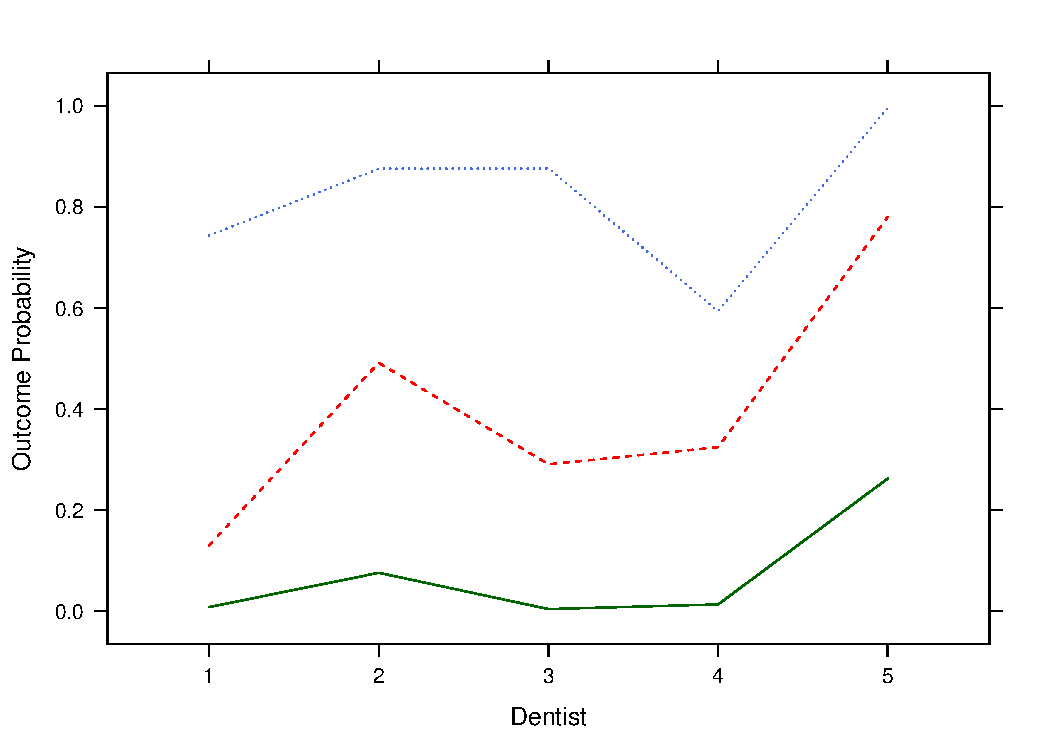
\includegraphics{randomLCA-example-014}
  \caption{Outcome probabilities for 3 Class Latent Class model.}
  \label{fig:outcome3}
\end{figure}

\begin{figure}
  \centering
\begin{Schunk}
\begin{Sinput}
> trellis.par.set(col.whitebg())
> print(plot(dentistry.lca2,type="l",xlab="Dentist",
+     ylab="Outcome Probability"))
\end{Sinput}
\end{Schunk}
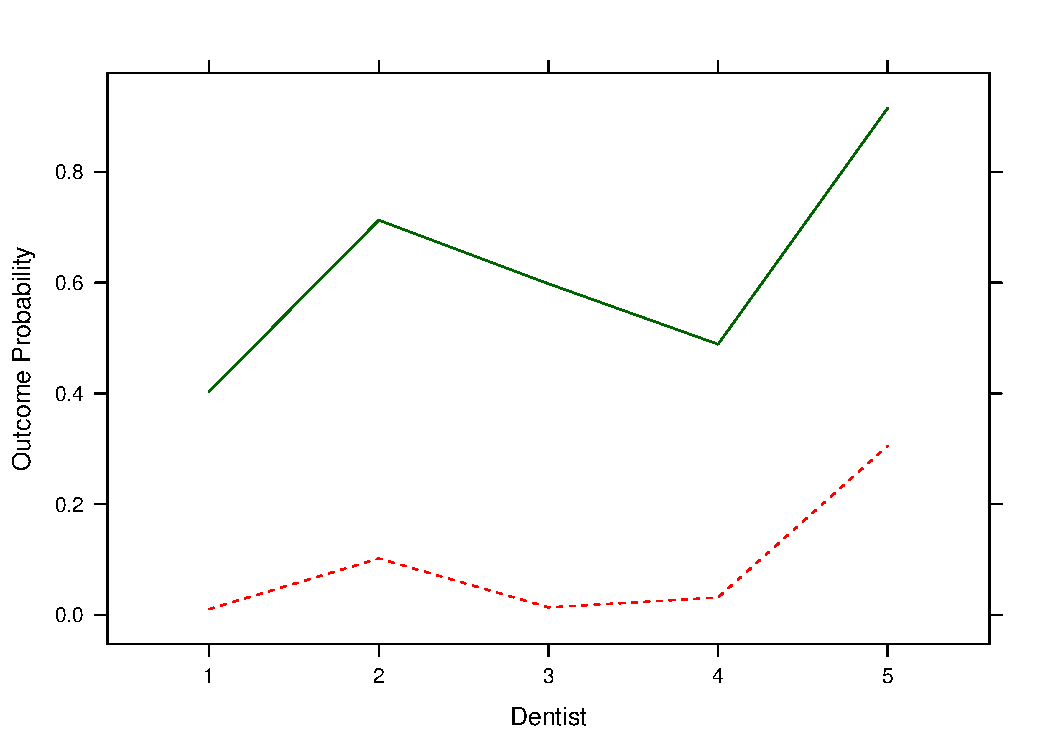
\includegraphics{randomLCA-example-015}
  \caption{Outcome probabilities for 2 Class Latent Class model.}
  \label{fig:outcome2b}
\end{figure}

The 2 Class results can be interpreted as a diagnostic test. Important results for diagnostic testing are the sensitivity and specificity for each test. The sensitivity is the probability of the test correctly identifying the subject as diseased given that the subject is diseased. In classical diagnostic testing the "true" status of a subject is known through use of a "gold standard" which is assumed to, sometiems optimistically, correctly classify the subject. The latent class method constructs a hypothetical standard, which has the disadvantage that this is not known with certainty but it allows correctly for any uncertainty in the underlying disease state. The other measure is specificity which is the probability of correctly identifying a subject as not diseased.
The sensitivities are then simply the outcome probabilities for the diseased class, Class 2 and the specificity one minus the outcome probabilities for the non-diseased class, Class 1. These can be obtained with 95\% confidence intervals using the outcomeProbs function.

\begin{Schunk}
\begin{Sinput}
> outcomeProbs(dentistry.lca2)
\end{Sinput}
\begin{Soutput}
Class  1 
    Outcome p       2.5 %     97.5 %
V1 0.01061849 0.006938943 0.01621734
V2 0.10198791 0.089733840 0.11570269
V3 0.01359123 0.008593070 0.02143371
V4 0.03156301 0.024211341 0.04105307
V5 0.30527875 0.287119234 0.32406470
Class  2 
   Outcome p     2.5 %    97.5 %
V1 0.4033508 0.3616418 0.4465055
V2 0.7128814 0.6691330 0.7529807
V3 0.5981284 0.5494271 0.6449673
V4 0.4888448 0.4468921 0.5309552
V5 0.9154706 0.8856536 0.9380562
\end{Soutput}
\end{Schunk}

The sensitivity and specificity are shown in Table~\ref{tab:outcomeconfint}. A reasonable conclusion is that the dentists are fairly good at identifying teeth that are not diseased (except for dentist 5), but not too good at identifying teeth that are diseased.

\begin{Schunk}
\begin{Sinput}
> probs <- outcomeProbs(dentistry.lca2)
> # this swaps around the probabilities based on the knowledge that
> # the outcome probabilities are higher in the diseased class
> order <- ifelse(probs[[1]][1,1]<probs[[2]][1,1],2,1)
> spec <- NULL
> sens <- NULL
> for (i in 1:5) {
+     sens <- c(sens,sprintf("%3.2f (%3.2f,%3.2f)",probs[[order]]$Outcome[i],
+         probs[[order]]$"2.5 %"[i],probs[[order]]$"97.5 %"[i]))
+     spec <- c(spec,sprintf("%3.2f (%3.2f,%3.2f)",1-probs[[3-order]]$Outcome[i],
+         1-probs[[3-order]]$"97.5 %"[i],1-probs[[3-order]]$"2.5 %"[i]))
+ }
> stable <- data.frame(sens,spec)
> names(stable) <- c("Sensitivity","Specificity")
> row.names(stable) <- paste("V",1:5,sep="")
\end{Sinput}
\end{Schunk}

\begin{Schunk}
\begin{Sinput}
> print(xtable(stable, digits = c(0,2,2),
+ 	caption="Sensitivity and Specificity",
+ 	label="tab:outcomeconfint"),include.rownames=TRUE)
\end{Sinput}
% latex table generated in R 3.1.2 by xtable 1.7-3 package
% Mon Nov 17 10:15:19 2014
\begin{table}[ht]
\centering
\begin{tabular}{rll}
  \hline
 & Sensitivity & Specificity \\ 
  \hline
V1 & 0.40 (0.36,0.45) & 0.99 (0.98,0.99) \\ 
  V2 & 0.71 (0.67,0.75) & 0.90 (0.88,0.91) \\ 
  V3 & 0.60 (0.55,0.64) & 0.99 (0.98,0.99) \\ 
  V4 & 0.49 (0.45,0.53) & 0.97 (0.96,0.98) \\ 
  V5 & 0.92 (0.89,0.94) & 0.69 (0.68,0.71) \\ 
   \hline
\end{tabular}
\caption{Sensitivity and Specificity} 
\label{tab:outcomeconfint}
\end{table}\end{Schunk}


The confidence intervals for the outcome probabilities can be calculated using the parametric bootstrap. These are shown in Table~\ref{tab:outcomeconfintboot} and are in agreement with those from the standard errors.


\begin{Schunk}
\begin{Sinput}
> probs <- outcomeProbs(dentistry.lca2,boot=TRUE)
> # this swaps around the probabilities based on the knowledge that outcome probabilities are higher in the diseased class
> order <- ifelse(probs[[1]]$Outcome[1]>probs[[2]]$Outcome[1],1,2)
> spec <- NULL
> sens <- NULL
> for (i in 1:5) {
+ 	sens <- c(sens,sprintf("%3.2f (%3.2f,%3.2f)",probs[[order]]$Outcome[i],
+       probs[[order]]$"2.5 %"[i],probs[[order]]$"97.5 %"[i]))
+ 	spec <- c(spec,sprintf("%3.2f (%3.2f,%3.2f)",1-probs[[3-order]]$Outcome[i],
+       1-probs[[3-order]]$"97.5 %"[i],1-probs[[3-order]]$"2.5 %"[i]))
+ }
> stable <- data.frame(sens,spec)
> names(stable) <- c("Sensitivity","Specificity")
> row.names(stable) <- paste("V",1:5,sep="")
\end{Sinput}
\end{Schunk}

\begin{Schunk}
\begin{Sinput}
> print(xtable(stable, digits = c(0,2,2),
+ 	caption="Sensitivity and Specificity",
+ 	label="tab:outcomeconfintboot"),include.rownames=TRUE)
\end{Sinput}
% latex table generated in R 3.1.2 by xtable 1.7-3 package
% Mon Nov 17 10:15:42 2014
\begin{table}[ht]
\centering
\begin{tabular}{rll}
  \hline
 & Sensitivity & Specificity \\ 
  \hline
V1 & 0.40 (0.37,0.44) & 0.99 (0.98,0.99) \\ 
  V2 & 0.71 (0.67,0.75) & 0.90 (0.88,0.91) \\ 
  V3 & 0.60 (0.55,0.64) & 0.99 (0.98,0.99) \\ 
  V4 & 0.49 (0.45,0.53) & 0.97 (0.96,0.97) \\ 
  V5 & 0.92 (0.88,0.94) & 0.69 (0.68,0.71) \\ 
   \hline
\end{tabular}
\caption{Sensitivity and Specificity} 
\label{tab:outcomeconfintboot}
\end{table}\end{Schunk}


The true and false positive rates can be plotted for each dentist, and are shown in Figure~\ref{fig:truefalse}. This gives a better explanation of what is happening. It appears that the difference between dentists is mainly related to the threshold for what they classify as diseased. Dentist 5 is more likely to correctly identify teeth as diseased but at the expense of being more likely to identify non-diseased teeth as diseased.

\begin{Schunk}
\begin{Sinput}
> itpr <- ifelse(dentistry.lca2$classp[2]>dentistry.lca2$classp[1],1,2)
> ifpr <- 3-itpr
> probs <- outcomeProbs(dentistry.lca2)
> probs <- data.frame(tpr=probs[[itpr]][,1],fpr=probs[[ifpr]][,1])
\end{Sinput}
\end{Schunk}

\begin{figure}
  \centering
\begin{Schunk}
\begin{Sinput}
> trellis.par.set(col.whitebg())
> print(plot(tpr~fpr,type="p",
+ 	xlab="False Positive Rate\n(1-Specificity)",
+ 	ylab="True Positive Rate (Sensitivity)",data=probs))
\end{Sinput}
\begin{Soutput}
NULL
\end{Soutput}
\end{Schunk}
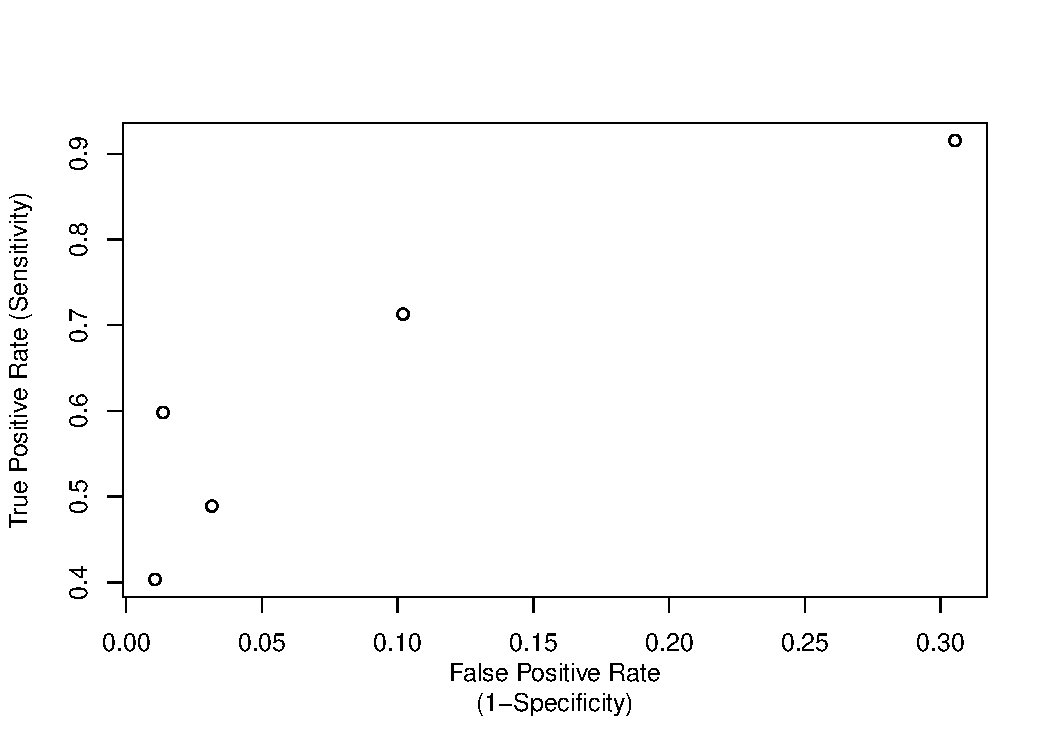
\includegraphics{randomLCA-example-022}
  \caption{True and False Positive Rates by Dentist.}
  \label{fig:truefalse}
\end{figure}

\section{Latent Class with Random Effects}

\subsection{Model}

The method used in \citet{qu:1996} is to introduce a random effect to model heterogeneity within classes. In their model the probabilities are transformed to the probit scale and then a normal random effect introduced. In practice it usually makes little difference if a probit or logit transform is used.

The probability for each observation remains the same, except that it is now conditional on both class $c$ and random effect $\lambda$.

\begin{eqnarray*}
P\left(y_{i1},y_{i2},...,y_{ik}|c,u\right)&=&\prod_{j=1}^k \pi_{cj}^{y_{ij}} \left(1-\pi_{cj}\right)^{1-y_j}\\
\end{eqnarray*}
Where
\begin{eqnarray*}
\pi_{cj}&=&\frac{e^{a_{cj}+b_ju}}{1+e^{a_{cj}+b_ju}},u\sim N(0,1)\\
\end{eqnarray*}
$b_j$ scales the random effect - models may have either a common or independent scale for each outcome, these are the \texttt{lambdacoef}. They may also be chosen to be different for each class, the default is for them to be the same for each class. \\

One way of visualising the model is that each class is now an Item Response Theory (IRT) model when the scaling is independent. When the scaling is common, the loadings are the same for each outcome and each class is then a Rasch model.

\subsection{Example 2 Continued}

We now continue the analysis of the dentistry data, allowing for random effects. This has a simple interpretation. For each subject there will be a different level of disease, and as a result a dentist will be more or less likely to classify the subject as having disease.



\begin{Schunk}
\begin{Sinput}
> dentistry.lca2random <- randomLCA(dentistry[,1:5],freq=dentistry$freq,
+ 	nclass=2,random=TRUE,quadpoints=41,probit=TRUE)
\end{Sinput}
\end{Schunk}

The BIC is reduced to 14944.7 showing an improvement over any of the latent class models. An alternative model is to allow the variance of the random effect to vary by outcome (dentist). This can be performed using the \texttt{constload} parameter. The default is true, so setting this to false allows the loading to vary for each outcome.

\begin{Schunk}
\begin{Sinput}
> dentistry.lca2random1 <- randomLCA(dentistry[,1:5],freq=dentistry$freq,
+ 	nclass=2,random=TRUE,probit=TRUE,quadpoints=41,constload=FALSE)
\end{Sinput}
\end{Schunk}

This increases the BIC to 14949.4, and is the 2LCR model obtained by \citet{qu:1996}. It appears that the simpler model is more appropriate.

A further extension is to allow the loading or random effect variance to vary by class.

\begin{Schunk}
\begin{Sinput}
> dentistry.lca2random2 <- randomLCA(dentistry[,1:5],freq=dentistry$freq,
+ 	nclass=2,random=TRUE,probit=TRUE,constload=FALSE,byclass=TRUE,
+   quadpoints=41)
\end{Sinput}
\end{Schunk}

The BIC increases to 14987.6. It is not surprising that this model isn't an improvement, there are now 21 parameters fitted to 32 observations. This also may give problems with the fitting algorithm so the number of quadrature points is increased to 41.

The marginal outcome probabilities, obtained by integrating over the random effect can be plotted, as in Figure~\ref{fig:outcome2}.



\begin{figure}
  \centering
\begin{Schunk}
\begin{Sinput}
> trellis.par.set(col.whitebg())
> print(plot(dentistry.lca2random1,graphtype="marginal",type="l",xlab="Dentist",
+     ylab="Marginal Outcome Probability"))
\end{Sinput}
\begin{Soutput}
NULL
\end{Soutput}
\end{Schunk}
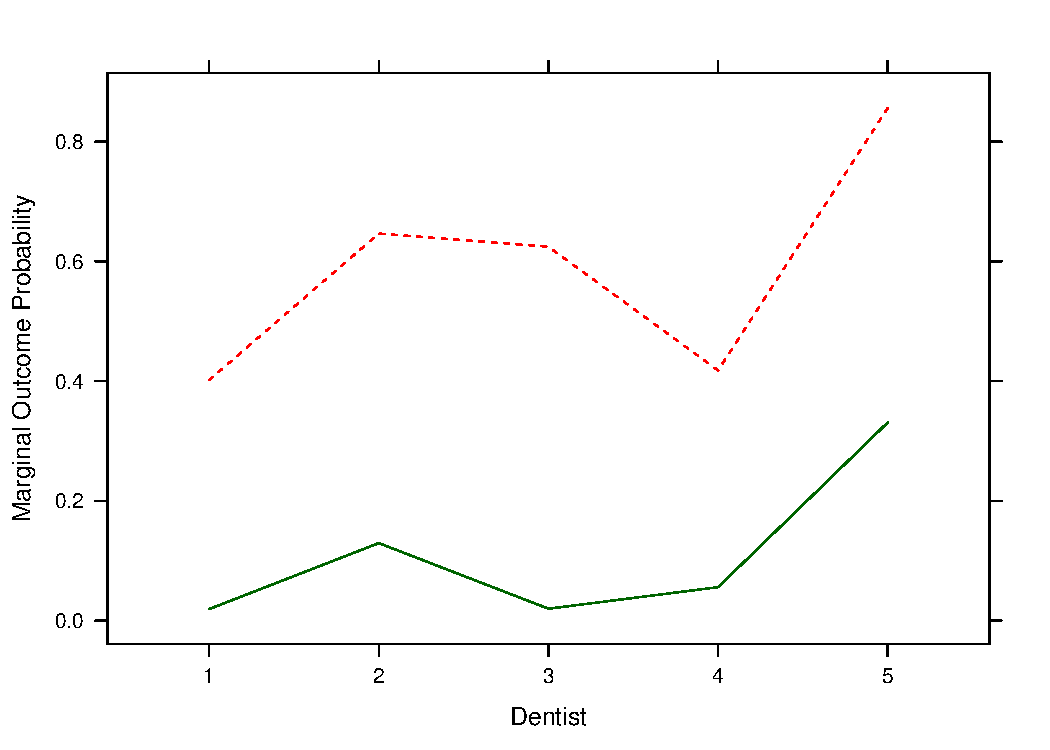
\includegraphics{randomLCA-example-026}
  \caption{Marginal Outcome Probabilities for 2 Class Latent Class with Random Effect (2LCR) model.}
  \label{fig:outcome2}
\end{figure}

Outcome probabilities with confidence intervals may be calculated for models with random effects only using the parametric bootstrap. The sensitivity and specificity may be obtained from these and are shown in Table~\ref{tab:outcomeconfintboot2}. Differences from the Qu et al paper result from them using a model with an individual loading for each dentist when calculating their Table 6.


\begin{Schunk}
\begin{Sinput}
> probs <-outcomeProbs(dentistry.lca2random,boot=TRUE)
> # this swaps around the probabilities based on the knowledge that outcome probabilities are higher in the diseased class
> order <- ifelse(probs[[1]]$Outcome[1]>probs[[2]]$Outcome[1],1,2)
> spec <- NULL
> sens <- NULL
> for (i in 1:5) {
+ 	sens <- c(sens,sprintf("%3.2f (%3.2f,%3.2f)",probs[[order]]$Outcome[i],
+       probs[[order]]$"2.5 %"[i],probs[[order]]$"97.5 %"[i]))
+ 	spec <- c(spec,sprintf("%3.2f (%3.2f,%3.2f)",1-probs[[3-order]]$Outcome[i],
+       1-probs[[3-order]]$"97.5 %"[i],1-probs[[3-order]]$"2.5 %"[i]))
+ }
> stable <- data.frame(sens,spec)
> names(stable) <- c("Sensitivity","Specificity")
> row.names(stable) <- paste("V",1:5,sep="")
\end{Sinput}
\end{Schunk}


\begin{Schunk}
\begin{Sinput}
> print(xtable(stable, digits = c(0,2,2),
+ 	caption="Sensitivity and Specificity",
+ 	label="tab:outcomeconfintboot2"),include.rownames=TRUE)
\end{Sinput}
% latex table generated in R 3.1.2 by xtable 1.7-3 package
% Mon Nov 17 10:23:50 2014
\begin{table}[ht]
\centering
\begin{tabular}{rll}
  \hline
 & Sensitivity & Specificity \\ 
  \hline
V1 & 0.40 (0.33,0.47) & 0.98 (0.96,0.99) \\ 
  V2 & 0.65 (0.56,0.72) & 0.87 (0.85,0.89) \\ 
  V3 & 0.62 (0.32,0.84) & 0.98 (0.80,1.00) \\ 
  V4 & 0.42 (0.35,0.49) & 0.94 (0.93,0.96) \\ 
  V5 & 0.86 (0.78,0.91) & 0.67 (0.64,0.70) \\ 
   \hline
\end{tabular}
\caption{Sensitivity and Specificity} 
\label{tab:outcomeconfintboot2}
\end{table}\end{Schunk}

The observed and fitted values can be obtained and are shown in Table~\ref{tab:obs}. Differences from the Qu et al paper again result from their different model.

\begin{Schunk}
\begin{Sinput}
> obs.data <- data.frame(dentistry.lca2random1$patterns,dentistry.lca2random1$observed,
+ 	dentistry.lca2$fitted,dentistry.lca2random1$fitted)
> names(obs.data) <- c("V1","V2","V3","V4","V5","Obs","Exp 2LC","Exp 2LCR")
\end{Sinput}
\end{Schunk}



% latex table generated in R 3.1.2 by xtable 1.7-3 package
% Mon Nov 17 10:23:50 2014
\begin{table}[ht]
\centering
\begin{tabular}{rrrrrrrr}
  \hline
V1 & V2 & V3 & V4 & V5 & Obs & Exp 2LC & Exp 2LCR \\ 
  \hline
0 & 0 & 0 & 0 & 0 & 1880 & 1836.3 & 1882.6 \\ 
  0 & 0 & 0 & 0 & 1 & 789 & 830.4 & 784.7 \\ 
  0 & 0 & 0 & 1 & 0 & 43 & 61.9 & 38.2 \\ 
  0 & 0 & 0 & 1 & 1 & 75 & 49.6 & 79.7 \\ 
  0 & 0 & 1 & 0 & 0 & 23 & 28.6 & 24.2 \\ 
  0 & 0 & 1 & 0 & 1 & 63 & 47.5 & 63.8 \\ 
  0 & 0 & 1 & 1 & 0 & 8 & 4.0 & 6.8 \\ 
  0 & 0 & 1 & 1 & 1 & 22 & 35.1 & 25.8 \\ 
  0 & 1 & 0 & 0 & 0 & 188 & 213.9 & 184.7 \\ 
  0 & 1 & 0 & 0 & 1 & 191 & 152.2 & 192.5 \\ 
  0 & 1 & 0 & 1 & 0 & 17 & 12.1 & 23.1 \\ 
  0 & 1 & 0 & 1 & 1 & 67 & 61.0 & 67.2 \\ 
  0 & 1 & 1 & 0 & 0 & 15 & 11.2 & 12.5 \\ 
  0 & 1 & 1 & 0 & 1 & 85 & 91.6 & 87.4 \\ 
  0 & 1 & 1 & 1 & 0 & 8 & 8.1 & 7.1 \\ 
  0 & 1 & 1 & 1 & 1 & 56 & 86.4 & 50.8 \\ 
  1 & 0 & 0 & 0 & 0 & 22 & 21.2 & 18.5 \\ 
  1 & 0 & 0 & 0 & 1 & 26 & 25.2 & 27.9 \\ 
  1 & 0 & 0 & 1 & 0 & 6 & 2.1 & 4.8 \\ 
  1 & 0 & 0 & 1 & 1 & 14 & 16.1 & 16.0 \\ 
  1 & 0 & 1 & 0 & 0 & 1 & 2.5 & 2.3 \\ 
  1 & 0 & 1 & 0 & 1 & 20 & 24.7 & 19.7 \\ 
  1 & 0 & 1 & 1 & 0 & 2 & 2.2 & 1.8 \\ 
  1 & 0 & 1 & 1 & 1 & 17 & 23.5 & 14.5 \\ 
  1 & 1 & 0 & 0 & 0 & 2 & 6.0 & 7.3 \\ 
  1 & 1 & 0 & 0 & 1 & 20 & 42.0 & 19.8 \\ 
  1 & 1 & 0 & 1 & 0 & 6 & 3.7 & 4.7 \\ 
  1 & 1 & 0 & 1 & 1 & 27 & 39.3 & 22.4 \\ 
  1 & 1 & 1 & 0 & 0 & 3 & 5.7 & 2.7 \\ 
  1 & 1 & 1 & 0 & 1 & 72 & 61.1 & 69.6 \\ 
  1 & 1 & 1 & 1 & 0 & 1 & 5.4 & 3.2 \\ 
  1 & 1 & 1 & 1 & 1 & 100 & 58.4 & 103.0 \\ 
   \hline
\end{tabular}
\caption{Observed and expected frequencies} 
\label{tab:obs}
\end{table}
